% !TEX root = slides.tex
%==============================================================================
\begin{frame}[t]
\label{merr2}

\frametitle{Model error -- General setup}
\vspace*{2mm}

%\bi
%\setlength{\itemsep}{0.2in}
%\setlength{\itemindent}{-.2in}
%\item
\textbf{Benchmark `true' model:} multiple output QoIs $g=(g_1,\dots,g_N)$
\bi
\item The same QoI at various operating conditions
\item The same QoI along a `cut' $g_i=g(x_i)$
\item Different QoIs, e.g. Pressure $g_1$, Temperature $g_2$, etc., or
\item \ldots a combination of above
\ei
%\item
\vspace{0.7em}
\textbf{Low-fidelity model:} matching output QoIs $f(\lambda)=(f_1(\lambda),\dots,f_N(\lambda))$
%\vspace*{-0.4cm}
\bi
\item Includes input parameter vector $\lambda$
\item Can have more outputs for `extrapolative' predictions $f_{N+1}(\lambda), \dots$
\ei
%\item
\vspace{0.7em}
\textbf{Goal:} calibrate $f(\lambda)$, such that
%\vspace*{0.4cm}
\centerline{$\qquad$
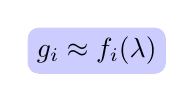
\begin{tikzpicture} \node [rounded corners,fill=blue!20] {
$g_i \approx f_i(\lambda)$
};
\end{tikzpicture}
}
%\vspace*{-0.9cm}
%\item
\vspace{0.5em}
\textbf{Challenge:} requires statistical model to
capture discrepancy $g_i-f_i(\lambda)$
%\vspace*{-0.4cm}
%\item
\bi
\item explicit modeling QoI-specific, and may violate physical
  constraints
  \ei
%\ei
\end{frame}
%==============================================================================
